% -*- mode: Latex -*-
% Time-stamp: "2015-02-18 17:55:40 sb"

\documentclass[twocolumn,aps,pra,showpacs,preprintnumbers,bibnotes]{revtex4-1}

\usepackage[T1]{fontenc}

\usepackage{natbib}
\usepackage{graphicx}
\usepackage{bm}
\usepackage{color}
\usepackage{amsmath}

%% Keep track of changes
%\usepackage[final]{changes}
\usepackage[draft]{changes}
\definechangesauthor[color=green]{AM}
\definechangesauthor[color=blue]{SB}

\DeclareMathOperator{\re}{Re}
\DeclareMathOperator{\im}{Im}

\newcommand\avg[1]{\left\langle#1\right\rangle}

\newcommand\unit[2]{\ensuremath{#1~\mathrm{{#2}}}}

\newcommand\Ket[1]{\ensuremath{|{#1}\rangle}}
\newcommand\Bra[1]{\ensuremath{\langle{#1}|}}

\newcommand\Isotope[2]{\ensuremath{^{#1}\mathrm{#2}}}
\newcommand\Li{\Isotope{6}{Li}}
\newcommand\K{\Isotope{40}{K}}
\newcommand\Rb{\Isotope{87}{Rb}}
\newcommand\Sr{\Isotope{87}{Sr}}
\newcommand\Yb{\Isotope{171}{Yb}}
\newcommand\Er{\Isotope{167}{Er}}
\newcommand\Dy{\Isotope{161}{Dy}}

\renewcommand{\vec}[1]{\ensuremath{\bm{#1}}}

\newcommand\NA{\ensuremath{\mathrm{NA}}}
\newcommand{\osim}{\ensuremath{\mathord{\sim}}}
\newcommand{\Erecl}{\ensuremath{E_\mathrm{rec}}}
\newcommand{\Ereca}{\ensuremath{E_\mathrm{rec}^\mathrm{(a)}}}
\newcommand\FIXME{{\color{red}\ensuremath{\mathrm{FIXME}}}}

\newcommand\TrapFreq{\ensuremath{\nu_t}}
\newcommand\RecoilEnergy{\ensuremath{E_\mathrm{rec}}}

\graphicspath{{./figures/}}
\begin{document}

\title{Design and Implementation of Stable High Power Optical Lattices for Quantum Gas Microscopy}


\author{Li Microscope Collective}
\author{M. Greiner}
\affiliation{
  Department of Physics, Harvard University,
  Cambridge, Massachusetts, 02138, USA}

\date{\today}
\begin{abstract}
We describe the design of a stable high power 1064 nm laser for use in optical lattice experiments. The system is based on a high quality mephisto NPRO seeding an array of four heavily modified fiber amplifiers. The intensity of every beam is stabilized with a low noise, nonlinear feedback system, and the waist can be smoothly controlled. 
\end{abstract}
\maketitle

\section{Introduction}
Ultracold atoms in optical lattices have become a powerful platform for experiments ranging from investigations of strongly correlated systems, quantum state engineering, quantum computing architectures, and precision metrology.
Further, the recent advent of quantum gas microscopy has enabled studies that exhibit unprecedented control over few atom systems at extremely low energy scales.
However, this rapid progress places ever more stringent technical constraints on the lasers used to trap and manipulate the atomic systems.
For example, heating due to the intensity noise of any laser cannot be allowed to approach the longest thermalization timescales, lest the system fail to thermalize~\cite{Savard1997}. 
Since thermalization timescales generally grow with falling temperature, this complicates attaining low temperatures.
Similarly, experiments that rely on a small number of atoms held by multiple traps places stringent requirements on the relative positional stability of the traps, to ensure that the operations performed by the traps have adequate fidelity.

In this note, we describe a high power optical lattice system that exhibits levels of intensity noise below $-120\,$dBc between $1\,$kHz and $3\,$MHz.
It also exhibits positional stability of the lattice phase at the $<0.5\,\mu$m level and of the harmonic confinement at the few site level over the course of hours.

The architecture of the system is based on a single low-power, low-noise seed laser (Innolight Mephisto) that supplies light to an array of four high-power fiber amplifiers (one for a transport beam~\cite{Huber2014}, and one each for the $X,Y,Z$ lattices)\cite{Parsons2015}.
Each fiber amplifier (Nufern NuAmp SUB1174-34) provides approximately 30 W, required to attain sufficient trap frequencies.
The fiber amplifier output is controlled by two feedback loops which stabilize the light in the low power and high power regimes.
After stabilization, the laser is mode-shaped to produce a desired waist when focused in the atom plane. 
Just before the beam is launched toward the atoms, a small sample of it is imaged by a camera to monitor the pointing.

To avoid interference effects among the lattice axes, AOM's are used to detune the fiber amplifier seeds away from each other.
These amplifiers can amplify 150 mW of seed light to up to approximately 45 W at the expense of dramatically raised levels of noise. 
The noise stems partially from stimulated Brillouin scattering, which is intrinsic, and several technical sources, which are not.

The NuAmp suffers from several problems: it is controlled via a USB interface, which is suspected to cause ground loops which add noise and interference to the analog systems, as seen in figure \ref{fig:noises}.
We solve this problem by replacing the USB control board with a custom solution that is compatible with our custom control system and that carefully avoids ground loops. 
There are two power supplies in the fiber amplifier - a general purpose supply for the control electronics and first amplification stage and a high power current supply for the second stage. 
Despite the presence of a water-cooled cold-plate to cool the optical fiber and pump diodes, the high power supply is air cooled using a fan approximately $20$ cm away from the gain fiber. 
This fan is suspected to lead to increased noise at acoustic frequencies.
In order to reduce acoustic coupling and reduce switching power supply noise, both power supplies were removed from the fiber amplifier chassis, and the low power supply was replaced by a linear PSU (Acopian A24MT350M). 
Further, a high current line filter (MPE DS26387) was added to the high-power PSU (Lumina LDD-600-60-10-5VP/M).
Combined, these changes serve to suppress many of the noise spurs measured in the RIN of the fiber amplifier, as seen in figure \ref{fig:noises}. 
The measurements in parts (a)-(d) were carried out on a single fiber amplifier, prior to and after the modifications. The initial and final noise spectra were verified to be consistent between amplifiers coming from the same manufacturing batch.
The figure is based on fiber amplifiers from a relatively new batch, which, even in its unmodified configuration does not exhibit a large switching supply spur. 
This is not the case for certain older batches, where the spur is approximately 30 dB higher than the background.

The operation of the Nufern fiber amplifiers can be further optimized by finely controlling the cooling water required, which by tunes the wavelength of the light supplied by the diodes that optically pump the gain fiber.
Optimizing the temperature is advantageous because (1) the maximum output power of the fiber amplifier is increased due to the improved efficiency of the pump light and (2) the lifetime of the device is increased because less stray pump light needs to be absorbed when the pump light is separated from the desired light, reducing the thermal load on the system.

This is possible because the pump diodes are fixed directly to the water-cooling plate without additional temperature regulation.
Adding a Peltier TEC and regulating to the optimal wavelength is possible, but is technically difficult as it requires large cooling power of $\approx100$ W per each of the three pump diodes and carries the associated complexity of three feedback loops.
We use a single, dedicated heat exchanger (TermoTek P21518970) to supply cooling water to an array of four fiber amplifiers and tune the temperature such that the average power supplied by the amplifiers supplying the $X$ and $Y$ lattices is optimized, while simultaneously keeping the temperature of the amplifier well within a safe range.
Experimentally, we have found that more power can be gained by running the amplifiers at hotter temperature, but we have avoided doing this in an effort to increase the lifetime.
We have experimentally found that there is variation in the sensitivity to the cooling water temperature between fiber amplifiers. 

\begin{figure}
  \begin{center}
    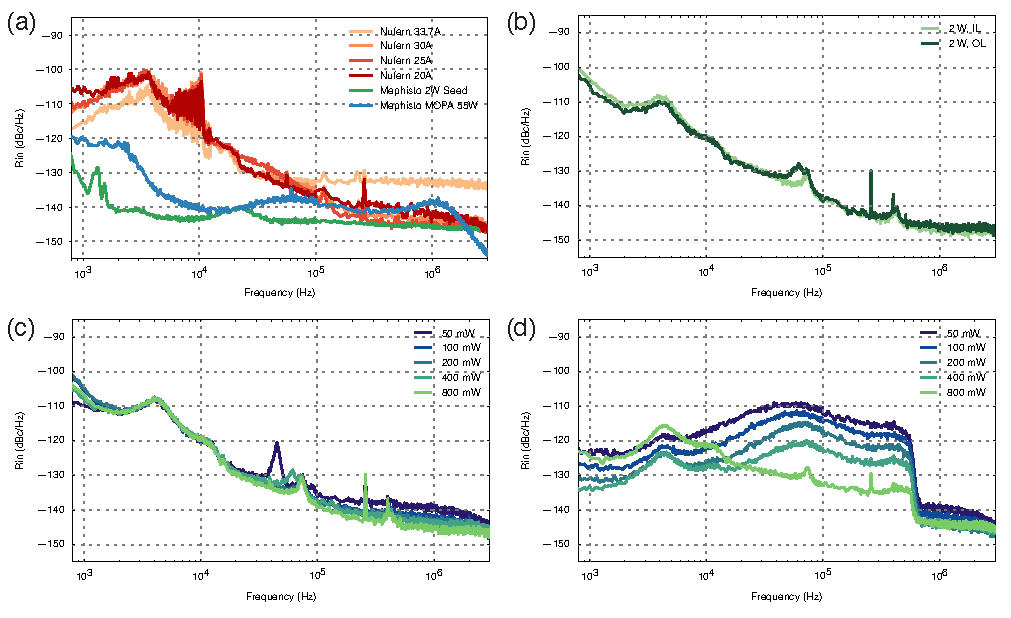
\includegraphics{fig/fig3_combined.pdf}
    \caption{\textbf{Laser noise of the lattice system.} (a) Shows the laser noise of unmodified Nufern fiber amplifiers and the Mephisto seed. (b) Shows the open (OL) and closed (CL) loop behavior of the high power feedback loop. (c) Shows open loop behavior of the low power feedback loop after making the modifications. (d) Closed loop behavior of the loop system without additional filtering, measured on the same setup as (c).}\label{fig:noises}
  \end{center}
\end{figure}


\subsection{Mode and beam shaping}

\begin{figure}
  \begin{center}
    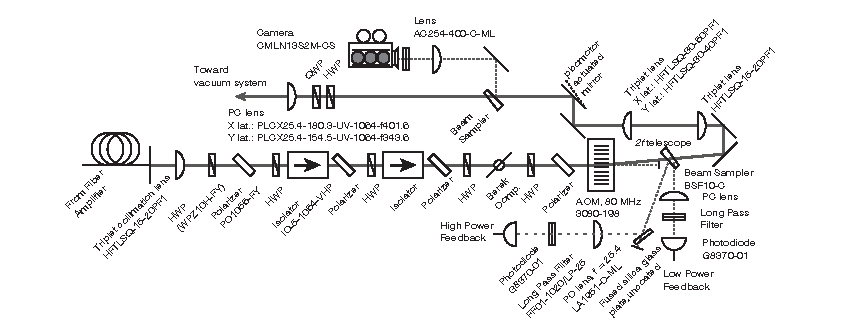
\includegraphics{fig/optical_layout_wide.pdf}
    \caption{\textbf{Optical layout of the optical lattice system for beam shaping and modulation.}}\label{fig:optical_layout}
  \end{center}
\end{figure}

The free-space propagation of the fiber amplifier output presents several technical challenges:
\begin{enumerate}
  \item The high optical power poses a significant danger to users and equipment.
  \item The high optical power is sufficient to induce substantial thermal lensing in some optics. 
  \item The positional fluctuations of the waist at the atoms cannot be allowed to exceed a few microns from shot to shot. 
\item By construction, the beam is retro-reflected, threatening the lifetime of the amplifier unless sufficient isolation is used. 
\item Approximately $1$ W of power leaks into the undesired cladding modes of the fiber. 
  \end{enumerate}

In order to address these challenges, we carefully engineered an optical system, shown in figure \ref{fig:optical_layout}, that cleans up the beam, controls its intensity between $10\,\mu$W and $20$ W, and ensures good pointing stability.
Due to the high laser power, fused silica glass is used wherever possible.
%except in the acousto-optic modulator (which is TeO$_2$), Berek compensator (which is quartz), and optical isolators, to minimze thermal lensing.
For the same reason, IBS coatings are used wherever possible, due to the higher damage thresholds.
Further, even small reflections pose both a danger to the users and risk damaging cables or starting a fire, so to alleviate this danger, all undesired beams above $100$ mW are directed to water cooled beam-dumps, which are placed as far as possible from critical beam paths. 
Weaker beams are dumped on uncooled diffusive beam catchers.

The large-diameter fiber tip at the output of the fiber amplifier is mounted in a monolithic mount made from oxygen-depleted copper.
The beam is collimated using an $f=20$ mm fused-silica, air-spaced triplet collimator (Opto-Sigma HFTLSQ-15-20PF1).
Then, the polarization is cleaned up using an IBS coated thin-film plate polarizer (Precision photonics PO1056-FY), which has the added benefit of rejecting the undesired cladding modes. 
The fact that the lattice is retro-reflected, combined with the observation that optical isolation falls with applied optical power~\cite{Yoshida1999} means that two stages of optical isolators must be used. 
The optical isolators are based on $5$ mm diameter isolators from Thorlabs (IO-5-1064-VHP), with the default cube polarizers replaced by IBS coated thin-film plate polarizers. 
Since the isolators are located approximately $1$ m away from the ultracold atomic system, undesired stray fields can have a dramatic effect.
To overcome this problem the isolators are enclosed in mu-metal shielding.

\subsection{High power feedback}

After the beam has been cleaned up and isolated, it is important to consider two aspects of the desired experiment: 
\begin{enumerate}
\item The lattice power must be continuously tunable from around $10$ $\mu$W to around $20$ W. 
\item The location of the minimum Gaussian beam waist must be accurately positioned to overlap the other lattices and dipole traps present in the experiment, and must remain there for the duration of the collection process (hours to days).
\end{enumerate}
To satisfy the first of these requirements, a two-stage feedback system is implemented. The reason for the two stages is simple: the experiment typically operates in one of two regimes, which we will term \textit{detection} and \textit{interaction}. 
In the interaction phase of the experiment, the lattice is relatively shallow ($\approx 100-200$mW, corresponding to depths of $\approx 10 E_R$, where $E_R$ is the geometric recoil of the lattice), allowing atoms to tunnel and interact with other atoms. 
In this regime, fine and potentially fast control is required.
In the detection phase, the depth of the lattice is dramatically raised ($\approx 2000 E_R$), isolating atoms in their individual wells so that Raman sideband imaging can be performed~\cite{Parsons2015}.
In the detection regime, the control need not be fast, and the passive stability of the Mephisto laser ensures that noise is low at relevant frequency scales ($\approx 2$ MHz).
Thus, two loops are utilized, a fast loop that uses an acousto-optic modulator to actuate the laser power at low powers, and a slow loop which uses a Berek compensator, to actuate in the high power mode.

After the isolation stage, we use the sequence of optical elements shown in figure \ref{fig:optical_layout}, consisting of a polarizer, half-wave plate (HWP), Berek compensator mounted on a precision galvo (Thorlabs GVS002, or Camtech 8320K, depending on beam path) half-wave plate, and polarizer. 
The Berek compensator is a simple $z$-cut quartz plate coated to be anti-reflecting at 1064 nm. 
By tilting the plate about its vertical axis, the extraordinary axis is mixed into the propagation of the beam, leading to a tilt-dependent bi-refringence that can be tuned from a zero-wave plate past a half-wave plate.
Combined with the subsequent polarization optics, rotation of the Berek compensator changes the transmitted power with perfect contrast and transmitted power as a function of the tilt angle is shown in figure \ref{fig:berek}.

Full modulation contrast is achieved when the fast axes of the waveplates around the Berek compensator $\theta$ are at $22.5^\circ$ to the rotation axis of the Berek compensator.
In that case, if the Berek compensator does not change the polarization, the light is fully transmitted. 
If it functions as a half-wave plate, the light is fully rejected, with a smooth crossover between the two cases as the Berek angle, $\phi$, is adjusted.
This contrast can be reduced by varying $\theta$, to the limiting case where $\theta=0$, where the rotation of the Berek compensator does nothing, since the polarization of the light is parallel to the rotation axis of the quartz.

\begin{figure}
  \begin{center}
    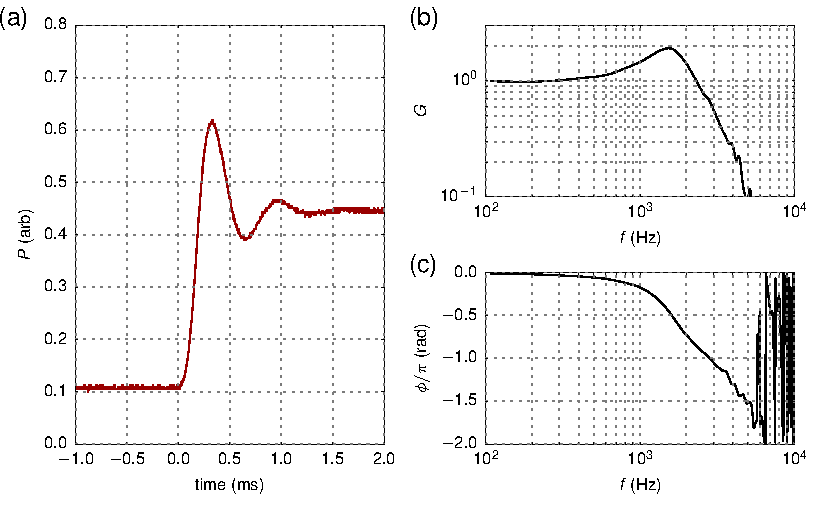
\includegraphics{fig/step_response.pdf}
    \caption{\textbf{Berek compensator based feedback loop} performance showing the impulse response (a) at relatively low powers and the corresponding Bode plots (b-c).}\label{fig:berek_step_response}
  \end{center}
\end{figure}
A key point is that, as seen in figure \ref{fig:berek}, if the two waveplates are rotated together, the maximum transmitted power is fixed, while the minimum can be raised.
The waveplates are detuned such that the maximum power needed in \textit{interaction} mode is the minimum power transmitted by the Berek compensator system, strongly suppressing fluctuations due to angle positioning noise of the Berek compensator. 
Naturally, rotation of a parallel plate in the beam path induces a shift of the beam, but this is acceptable because the Berek compensator is only active during the imaging phase of the experiment, when the position of the underlying harmonic trap is largely irrelevant.
Fortunately, the spatial phase of the optical lattice is set by the retro-reflector mirror, which does not move, and is not affected by the rotation of the Berek compensator.
This system functions as the actuator arm of a feedback loop, where the power of the beam is measured using a low noise photodiode. This feedback loop regulates the lattice between $1$ W of optical power and its maximum value (which depends on the amplifier, but is $\approx20$ W).
The step response and corresponding Bode plots~\cite{Bechhoefer2005} are shown in figure \ref{fig:berek_step_response}.
A polarization rotation by $2 \pi$ is produced by approximately $3^\circ$ of axial rotation of the quartz plate. 
Since we never need to rotate the plate outside this range, the position is constrained to this window in software.

\subsection{Low power feedback}
%The high power feedback used in the \textit{imaging} phase of the experiment and is exceedingly robust
%, and allows the user to raise the power and ensure an adequate Lamb-Dicke parameter\cite{Parsons2015}. 
The high power feedback used in the \textit{imaging} phase of the experiment is exceedingly robust because the heating rate from scattered resonant imaging light far exceeds any technical heating from the loop.
Even if the loop was designed by your worst enemy\footnote{I have received a number of comments about this particular statement. Yes, it was a hyperbole, and I concur - most likely readers of this thesis could design a system that would result in a heating rate exceeding the cooling, but you would definitely have to be malicious to do so.}, the heating would be entirely compensated by the simultaneous Raman cooling~\cite{Parsons2015}.

In contrast, the low power loop that controls the lattice laser during the \textit{interaction} phase of the experiment is critically important:
\begin{enumerate}
  \item Its RIN is one of the factors limiting the system temperature.
  \item It cannot affect the pointing.
  \item It must have closed loop bandwidths of $\geq1\mathrm{\,kHz}$, and open loop modulation bandwidths $\geq 100\mathrm{\,kHz}$.
\end{enumerate}
To this end, we use actuate the optical power using a TeO$_2$ AOM (Gooch \& Housego AOMO 3080-198), where the power of the RF supplied to the AOM is used to actuate the fast, low power feedback loop.
The AOM was chosen for its low thermal lensing and easily-accessible RF powers. 
It is mounted on a custom-built, monolithic, water-cooled flexure mount that allows optimization of the AOM efficiency, that has been found to remain stable over years of operation.

\begin{figure}
  \begin{center}
    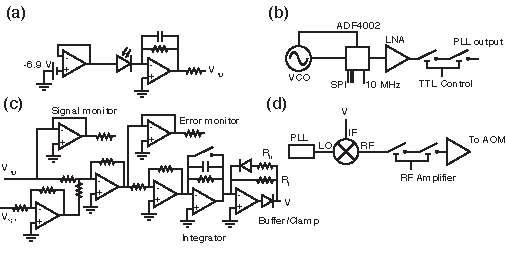
\includegraphics{fig/circuits.pdf}
    \caption{\textbf{Feedback circuits.} (a) The reverse-biased photodiode. (b) Externally referenced phase-locked loop. (c) Nonlinear loop filter. (d) RF power modulation using a mixer.}\label{fig:circuits}
  \end{center}
\end{figure}
The feedback circuit is shown in figure \ref{fig:circuits}a. A pair of low noise photodiodes measures the optical power of the beam sampled with a weakly reflective optic (Thorlabs BSF10-C). 
The beam sampler is wedged in such a way that the two reflections diverge from one another, allowing us to illuminate both photodiodes. 
One of the sampled beams is attenuated by a factor of $20\times$ by reflection off of an uncoated fused silica glass plate, such that the dynamic range of its photodiode covers $0-20$ W of the beam directed at the atoms, and controls the Berek compensator based, high-power, feedback loop. 
The other beam is not attenuated, save by the beam sampler, and its dynamic range covers $0-1$ W.
To prevent damage to this photodiode when the system is at its highest powers, a shutter (Stanford Research Systems SR475) blocks the light when the high power loop is active.
The low power photodiode passes its signal $V_{\mathrm{pd}}$ to a loop filter circuit, which compares it to the control system's set-point, generated by digital to analog converter.
The loop filter's output controls the IF port of a microwave mixer (Minicircuits ZFM-2-S+), effectively modulating the RF power supplied by a low noise phase-locked loop (PLL).
The resulting RF signal is then amplified and sent to the AOM.
Let us now consider every part of this signal chain individually.

\subsubsection{Phase-locked loop (PLL)}
The local oscillator (LO) RF source is a custom-built printed circuit board (PCB) implementing a phase locked loop (PLL) based on the ADF4002 IC and Crystek's CVCO55CL-0060-0110 voltage controlled oscillator (VCO), preamplified with a low noise amplifier (Minicircuits PSA4-5043+\footnote{This part has a plastic case which melts slightly if placed in a reflow oven, but still works as specified.}). 
To ensure frequency stability (which translates directly into beam pointing of the laser), the PLL is locked to the $10$ MHz clock distributed around the lab.
In addition to PLL functionality, the board also contains two, digitally-controllable, high-isolation RF switches, giving a total isolation exceeding $90$ dB.

The spectrum and relative intensity noise of the PLL can be found in figure \ref{fig:pll}. 
Vitally, the spectrum of the PLL exhibits phase noise comparable to that of typical VCO\footnote{Strictly speaking, a $-90$ dB phase noise is worse than specified. 
However, the measurement was carried out in ``peak detection'' mode on the spectrum analyzer, which artificially inflates the numbers by approximately 10 dB. 
This happens because the power at multiple frequency bands is measured within each frequency step on this plot, and in ``peak detection'', the highest is reported (all noise measurements in this work were carried out in ``RMS detection'', which is more suited for that purpose). The other reason that the phase noise appears worse than specified is that the dynamic range of the spectrum analyzer used is 100 dB, and we approach close to that limit.}, without the slow frequency drift characteristic to these devices.
Elimination of the carrier drift is worth the added phase noise because any drift of the frequency affects the steering of the laser beam passing through the AOM, which is entirely unacceptable since it would misalign the optical lattice.

\begin{figure}
  \begin{center}
    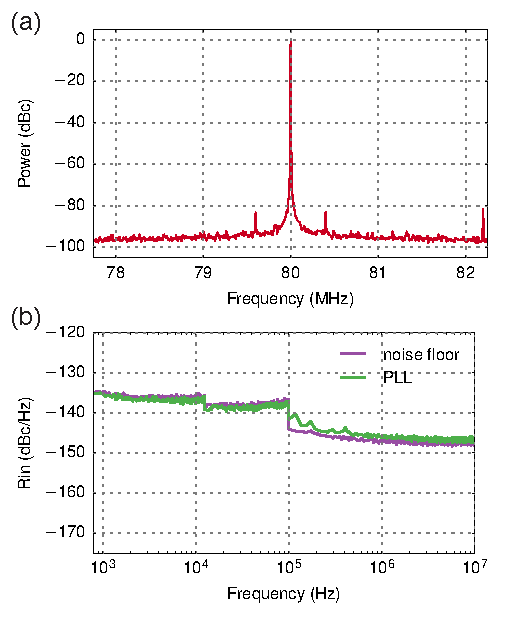
\includegraphics{fig/pll.pdf}
    \caption{\textbf{PLL performance} (a) The spectrum of the PLL, exhibiting phase noise of better than $-90$ dBc $100$ kHz away from the carrier. (b) The RIN of the local oscillator based on the PLL. The noise level is seen to be at or below the noise floor of the measurement device.}\label{fig:pll}
  \end{center}
\end{figure}

\subsubsection{Photodiode}

\begin{figure}
  \begin{center}
    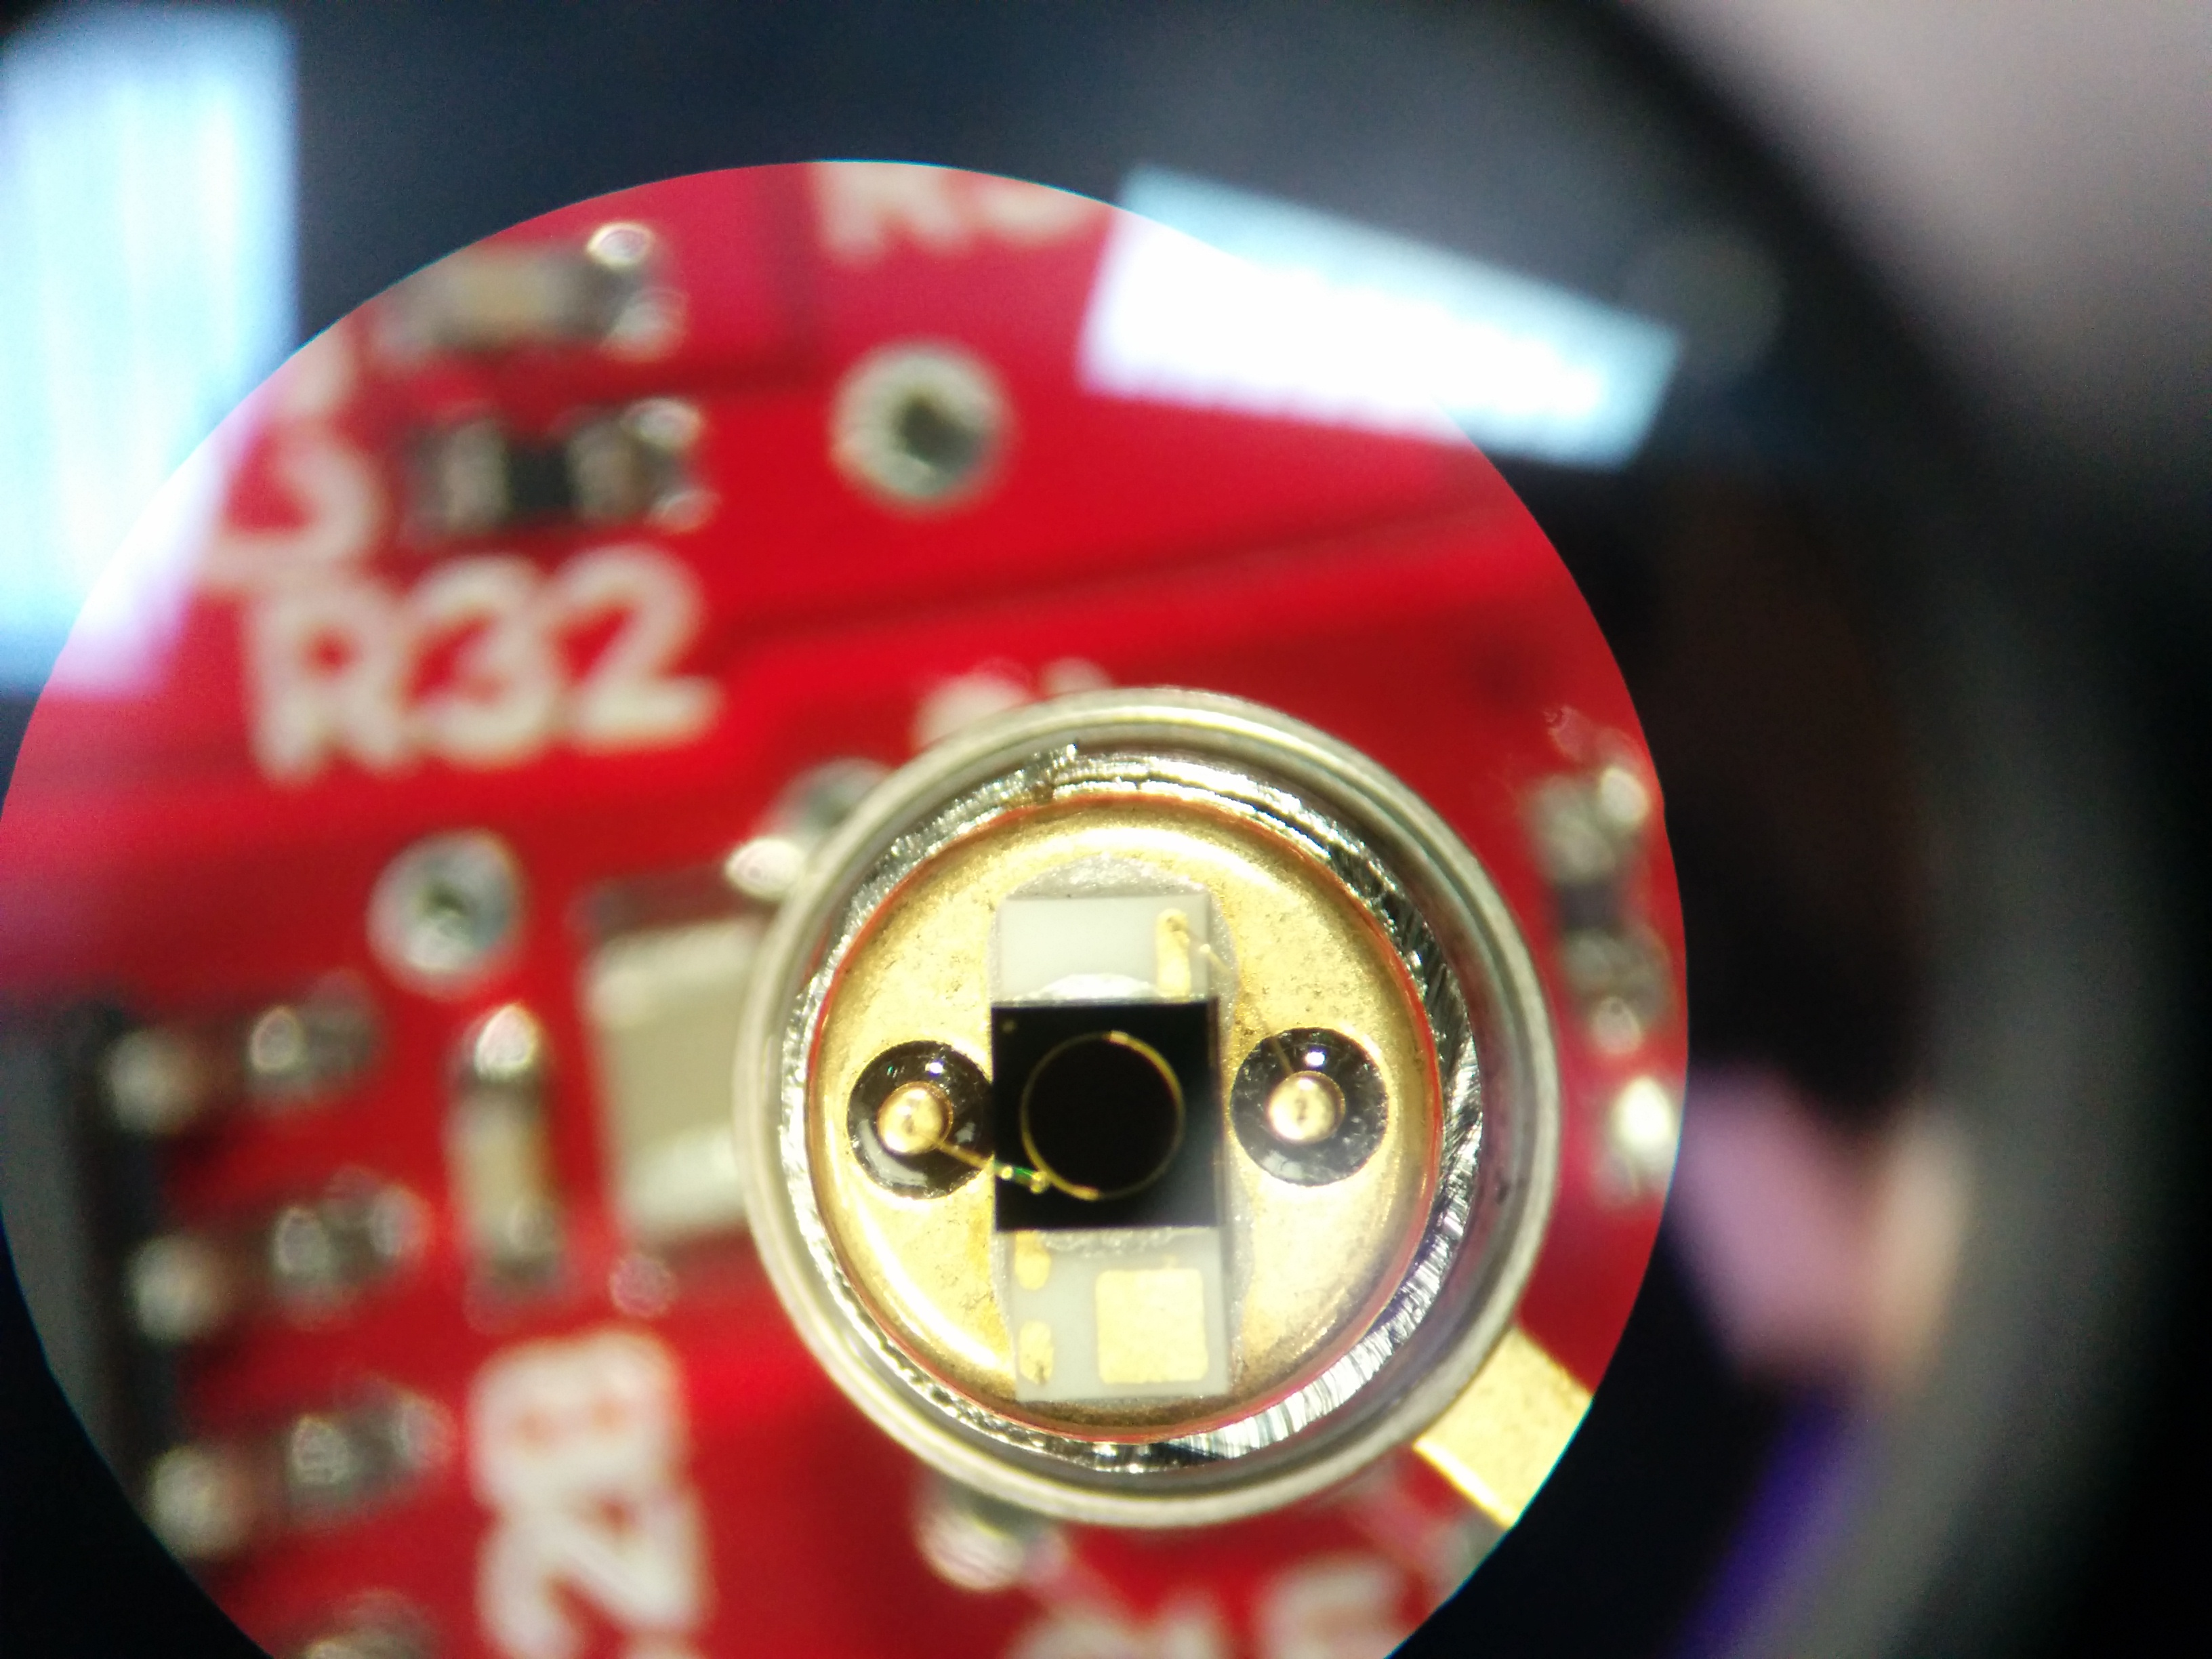
\includegraphics[scale=0.1]{fig/cut_photodiode.jpg}
    \caption{\textbf{Photodiode photo} showing that the ``can'' of the photodiode has been cut, to prevent etalon-like behavior.}\label{fig:cut_pd}
  \end{center}
\end{figure}

Fast, low-noise photodiodes are required both to provide the monitoring arm of the feedback loop and to characterize the RIN of the system.
An ideal device would have a bandwidth up to approximately 3 MHz\footnote{The maximum attainable trap frequencies in the system are around 1.5 MHz, and parametric heating is driven by $2\times$ the trap frequency}, with a noise floor below approximately -150 dBc over that range.
To approach these specifications, we use a custom designed PCB that implements a simple trans-impedance amplifier~\cite{Graeme1995} in a convenient physical package, providing a bandwidths in the 0.1-10 MHz range, depending on the trans-impedance gain set by a resistor. 
The photodiode can be safely operated up to incident powers of approximately 10 mW, which sets a -164 dBc/Hz shot noise limit on the RIN that can be detected. 
In practice, we typically operate the photodiodes with $\approx 5$ mW of incident power.
A photodiode with a bandwidth (BW) of 6 MHz is used to characterize the system, while photodiodes with a bandwidth of 330 kHz (and correspondingly higher gain) are used to perform the feedback.

The chosen photodiode (Hamamatsu G8370-01) is an InGaS based, small-area, low-noise design with a high efficiency at 1064 nm.
Prior to use, the protective window is removed from the photodiode to prevent interference effects, as seen in figure \ref{fig:cut_pd}.
Further, to reduce the capacitance of the system, a reverse bias of 6.9 V is applied to the photodiode by a temperature-stabilized voltage reference (Linear Technology LM399).
The trans-impedance circuit is shown in figure \ref{fig:circuits}. 
It converts the photo-current supplied by the photodiode to a voltage signal using the low noise Texas Instruments OPA843 op-amp. 
To reduce electrical pickup and prevent ground loops, the electronic assembly is housed in a metal enclosure and mounted to the optical table using electrically insulating mica posts. 

Light is focused onto the photodiode using a 25.4 mm lens such that the beam at the photodiode is significantly smaller than the photodiode diameter, to prevent pointing fluctuations from registering as amplitude fluctuations. 
An iris and interference filter (Semrock FF01-1020/LP25) are used to eliminate stray sources of light. 


\subsubsection{Digital to analog converter}
The digital to analog converter (DAC, Texas Instruments DAC9881) connects the experimental digital control system to the analog control loop for the lattice. 
By definition, an ideal control loop would translate any noise on the analog signal from the DAC to the laser light, meaning that a poorly designed DAC would inherently limit the lattice laser performance.
The noise on the DAC, when it is programmed to output a constant voltage is shown in figure \ref{fig:da_rin}, and is found to be roughly constant at a level of $-150$ dBc - more than acceptable.
When the state of the DAC is changed, such as during a ramp, this noise level may be higher, due to the so-called ``glitch'' energy, as seen in the figure.
The transient noise, while unfortunate, is mitigated by two factors: (1) it is only present when the lattice power is altered, which happens during lattice loading - a lattice at a fixed power will have negligible RIN contributions from the DAC. Further, (2) the loop filter will filter the noise at these frequencies. 

\begin{figure}
  \begin{center}
    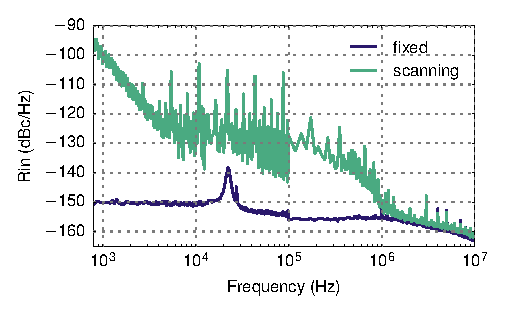
\includegraphics{fig/da_rin_scan.pdf}
    \caption{\textbf{Relative intensity noise of the digital to analog converter} at a fixed output voltage and while changing values. To measure the transient RIN, a $20$ ms, triangle wave with a DC offset and modulation depth of $15$\% of the DC offset was produced by the device. The triangle wave accounts for the series of spurs at low frequencies that fall with increasing frequencies. At frequencies above approximately $4$ kHz, the spectrum is dominated by noise due to transient ``glitches'' that emerge when the device changes its output state.}\label{fig:da_rin}
  \end{center}
\end{figure}


\subsubsection{Loop filter}

The connection between the actuation and monitoring mechanisms of the feedback system is the loop filter, which compares the \textit{set-point} signal, $v_s(t)$, supplied by the experimental control system and the monitoring signals $v_m(t)$, to adjust the actuation accordingly.
We use a simple, purely integrating design based in three stages, as seen in figure \ref{fig:circuits}, based on TI's OPA211 op-amp.
The first stage computes and amplifies an error signal, $e(t)=v_m(t)-v_s(t)$, which is integrated by the second stage. 
The integral gain is set using a low-drift trim-pot. 
This is the case because within relevant frequency ranges, the AOM can be well approximated by a pure time delay process (with delay given by the RF travel time across the crystal $\approx 1 \mu\mathrm{s}$).
In this scenario, the $P$ term must be small to avoid instability at the $\pi$ phase shift point, and a pure $I$ controller is optimal~\cite{Skogestad2001}.
For debugging purposes, the loop filter features buffered photodiode monitor and error signal monitor outputs.

The third stage of the loop filter is used to accommodate the fact that the actuation arm is in nonlinear - the optical power transmitted by the AOM is proportional to the RF power incident on it $P_{\mathrm{rf}}\propto v_{if}^2$, where $v_{if}$ is the actuation signal supplied to the IF port of the mixer.
In effect, if the rest of the feedback system was linear, this would correspond to a quadratically increasing gain until the AOM is saturated, which could lead to slow behavior at low signal levels and ringing at higher signal levels.
Even worse, since the mixer is insensitive to the sign of the voltage applied, the gain is actually negative for negative voltages, resulting in an unstable system, which thus requires a current clamp.
This stage linearizes the response by increasing the gain at low signal levels and suppressing it at high signal levels by using a diode (Digi-Key BAT54S) in the feedback arm.
This can be seen by considering two extreme cases - far below the diode drop, the diode is an open circuit and the gain is set by $R_l$, where above the diode drop it is a closed circuit where the gain is set by the resistor $R_h$. 
Naturally, the voltage drop over the diode is chosen such that it is approximately half the maximum desired signal level of the photodiode ($3.3$ V).
Although a large improvement, the bandwidth still varies over the dynamic range of the loop, but only by approximately a factor of two, as seen in figure \ref{fig:bandwidth}.
Were it not for the linearization, the gain of the mixer would change by $10\times$ over a dynamic range spanning two orders of magnitude.
Another function of the last stage is to clamp the voltage to be strictly $>0$, in order to prevent an unstable positive feedback behavior, which is done using diode clamp on the output arm~\cite{Horowitz2015}.
Last of all, since the mixer is a current driven device, the last stage of the feedback loop uses TI's OPA627 op-amp which is able to supply tens of mA of current at an output impedance of $50$ $\Omega$.

\begin{figure}
  \begin{center}
    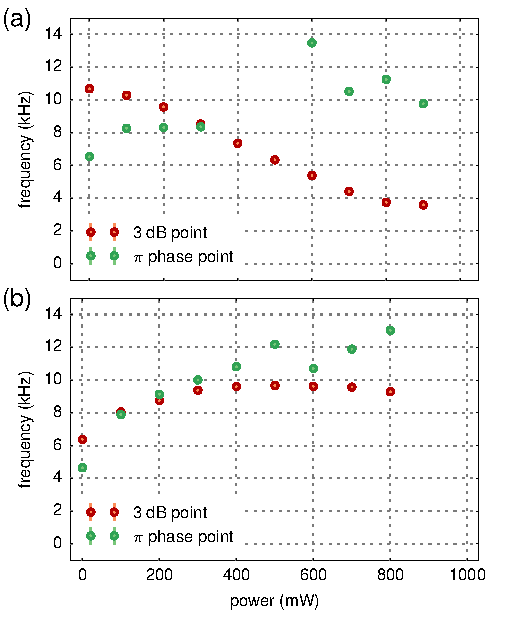
\includegraphics{fig/low_power_bandwidths.pdf}
    \caption{\textbf{Loop bandwidth dependence on the set-point}. (a) shows the $3$ dB and $\pi$ phase shift points for the $X$ lattice (also known internally as the ``northeast'' lattice. (b) shows the same for the $Y$ lattice, known as the ``northwest''.}\label{fig:bandwidth}
  \end{center}
\end{figure}


A common behavior of analog feedback systems with integration components is termed \textit{integral wind-up}~\cite{Bechhoefer2005}, and occurs when the feedback loop is manually broken, and the actuator can no longer adjust the state of the controlled parameter. 
In this regime, the integrator accumulates a large positive or negative value, such that when control is restored, the system is uncontrolled until the integrator reaches the desired value.
In our case, \textit{integrator wind-up} occurs when the high-isolation RF switch is open during the state preparation procedure, and closed when the lattice is desired. 
Since the lattice must usually be applied adiabatically, fast transients due to this windup can result in heating.
To solve this system, a bypass switch (Maxim MAX4503) is placed across the capacitor of the second stage of the feedback circuit, which siphons the charge off the capacitor when the lattice is inactive.
Even when the switch is closed, its resistance is nonzero (due to a protection resistor which limits the current that can pass through the switch), the conditions leading to integral windup in an unprotected system still lead to charge accumulation on the integral capacitor, albeit at a much reduced level.
Thus, in addition to the switch, when the system is inactive, the set-point is set to within ($\approx 200$ $\mu$V) of the dark signal from the photodiode, making the error signal very small.

To avoid a so-called ``servo bump'' in the noise spectrum, and because there is little need for fast, closed-loop control, the loop filter is tuned very conservatively, to a bandwidth of approximately 10 kHz over most of the range.
However, a small amount of tuning can raise this to up to $\approx150$ kHz, which is limited by the acoustic wave propagation delay of the AOM.
Although fast, closed-loop control is impossible in the current configuration, the last stage of the loop filter features an adder, connected to an optional ``feed-forward'' port, which can be used to modulate the RF power at frequencies above the bandwidth.

Although it is an essential part of the system, the loop filter is also one of its major limitations. Figure \ref{fig:noises} shows the noise performance of the output of the fiber amplifiers in open loop as compared to the noise in closed loop. Although noise near DC is lowered (as expected from a closed loop system), noise outside the loop bandwidth is increased in the range of $10$ to $450$ kHz as seen in subfigures (c) and (d).
This can be explained by the Johnson noise~\cite{Horowitz2015} on the $1$ k$\Omega$ input resistors, amplified by the amplification stages of the loop filter\footnote{This seems like a small quantity (-174 dBm), but there are several levels of amplification, and the voltage supplied to the mixer is small ($\approx 0.1 V$), all of which works against the experimentalist.}. 
The sharp drop off at the $450$ kHz point is due to the low-pass filter centered there, placed on the output of the loop filter.
When this was determined to be a problem, and we decided that a bandwidth of higher than $10$ kHz was not required in the near term, a first order low pass with a $3$ dB frequency of $10$ kHz, was also added, leading to the noise spectrum seen in subfigure (b), as compared to (a) in figure \ref{fig:low_pass_noises}\footnote{The fiber amplifier used to take this data was different from the one used for \ref{fig:noises} different fiber amplifiers, which explains the small discrepancies.}. 

\begin{figure}
  \begin{center}
    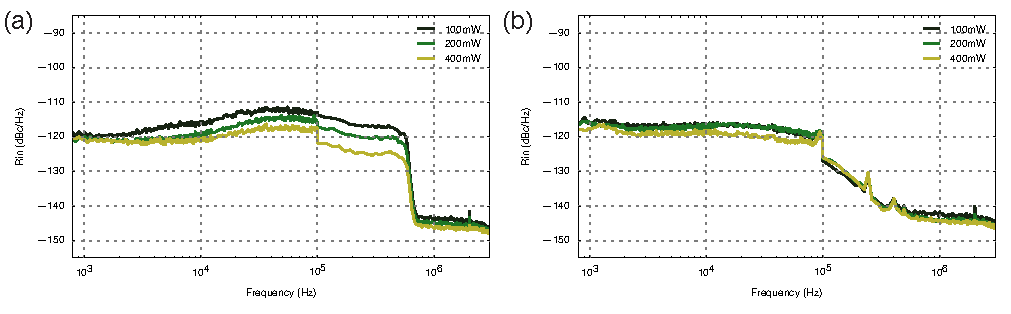
\includegraphics{fig/low_pass_filters.pdf}
    \caption{\textbf{Laser noise of the lattice system with and without additional low pass filters} (a) Closed loop laser made a fiber amplifier (different than the one in figure \ref{fig:noises}. (b) Noise on the same system as (a), but with extra filters.}\label{fig:low_pass_noises}
  \end{center}
\end{figure}


\subsubsection{Beam shaping}
After the beam has passed through the feedback optics, it must be applied to the atoms. To that end, we use a $2f$ telescope of short focal length triplet collimator lenses to expand the beam, and then focus it with a long focal length lens.
We focus the lattice to a $70-90$\,$\mu$m waist at the position of the atoms.
In order to verify that the waist is positioned correctly, we use a temporary mirror to redirect the beam away from the glass cell and onto a camera positioned in the plane that would correspond to the position of the atoms had it not been for the temporary mirror.
The resulting beam at the atoms has an $m^2\leq1.4$.

To prevent unwanted interference, the lattice beams enter the glass cell at an angle. 
Unfortunately, due to the angle of incidence, the beam contains both $S$ and $P$ polarizations, which are reflected differently, altering the polarization state of the beam.
Even worse, this happens on both the initial and retro-reflected pass through the glass cell.
For this reason, we use a QWP and HWP to optimize the interference contrast of each lattice\footnote{We do this by optimizing on the trap frequency of lattice, measured using parametric heating. This is a relatively tedious procedure.}.


\section{Beam monitoring and alignment}

Improved spatial resolution and control have given experimentalists the ability to use relatively few atoms~\cite{Preiss2015, Choi2016, Mazurenko2016} that are simultaneously addressed by multiple beams and held by multiple traps.
Such experiments place stringent bounds on the requisite stability. 

The absolute positions of lattice sites cannot be allowed to change by more than approximately $10\%$ from experimental shot to shot.
Fortunately, this is relatively straightforward to ensure via careful design of the optical assembly, since the phase of a retro-reflected lattice is set by the retro-reflecting mirror, which can be close to the position of the atoms and be made very stable~\cite{Huber2014}. 
We have characterized the phase stability of the optical lattice by looking at a long sequence of densely populated images, and found that the phase varies by much less than one lattice site over the course of hours.

The position of the atomic cloud, however, is not determined by the phase of the lattice, but by the underlying harmonic confinement, which, in turn, is determined by the positions of the ingoing and retro-reflected beams. 
In experiments where the entire cloud is addressed by beams auxiliary to the lattice (such as in this work, \cite{Mazurenko2016} or \cite{Choi2016}), drift or fluctuation of the lattice position can pose a severe limitation.

The required positional stability is achieved through a combination of passive stability and active monitoring. 
Passive stability is ensured by using stable optomechanics (from the Thorlabs Polaris line), mounted at a low ($2$ in) beam height relative to the floating optical table.
The beam is enclosed with aluminum tubes throughout its path and the entire setup is enclosed, to suppress air currents.

Passive stability alone has been found to be insufficient to ensure smooth operation over many hours because external factors can lead to a slow drift in the pointing of the laser beams. 
To address this concern, each lattice axis is fitted with a remotely actuated mirror connected to the control software.
The actuators are Newport brand ``Picomotors'' (model 8302), fitted into a customized $2$ in mirror mount.

\end{document}
